
\section{Motivation}

Do linguists need to spend long hours counting morphemes for measuring morpho-syntactic complexity? 
Ever since the first studies, \gls{mlu} plays an important role in language development investigations. 
This metric has been widely used for measuring linguistic productivity of children for almost a hundred years. 
Utterance lengths are usually calculated in morphemes (\acrshort{mlum}) being a time-consuming task. 
Even though CLAN toolkit \cite{MacWhinney1992} can count morphemes in utterances, this feature is only available just for a few languages not containing any agglutinative ones. %TODO: Kinga szerint az MLUm nem biztos, hogy usually

This chapter presents\footnote{This study is a joint work with Kinga Jelencsik-Mátyus. 
Manual annotation of the data were performed by both of us, while the morpheme counting principles are her work. 
My contribution is the construction of the tagging chain, its adaptation and the automatization of the MLUm calculation.} 
an automatic method for estimating \acrshort{mlum} for Hungarian transcripts. 
We show that PurePos can be used effectively for aiding linguists in this scenario. 
Our approach adapts this tagging tool (cf. Section \ref{sec:purepos}) yielding the first Hungarian tagger for spoken texts. 
Further on, we describe an \acrshort{mlum} estimation method, which is based on the latter tagger, resulting in a high quality output. 

First related studies are summarized, then we present resources used for the research. 
Next, the adaptation steps of PurePos are described and the framework designed is introduced. 
Finally, we show that both the tagger and the estimator methods are accurate enough to replace the labor-intensive manual calculation.

\section{Background}

Tagging approaches of spoken languages mainly cover only mainstream ones (such as English, Italian or Spanish) while agglutinative ones are usually neglected. 
One of the pioneers in this field was Eeg-Oloffson \cite{Svartvik1982} using  manually annotated transcripts to train a statistical tagger (for English). 
In contrast, there are others employing and adapting statistics of written language corpora \cite{Mendes2004,Nivre1996,Panunzi2004}.
Besides, building domain-specific rules also lead to satisfactory taggers (e.g. \cite{Moreno2003}),
while combination of such systems with stochastic tools \cite{Bick2012} yields effective algorithms as well. 

These previous studies imply that a proper morphological annotation system aiming to process transcripts must be able to handle the following types of difficulties:
\begin{enumerate}
 \item existence of new morpho-syntactic tags which are missing from the tagset of the training data,
 \item occurrence of tokens with non-standard orthography in texts,
 \item the number of words unknown to a statistical tagger are increased compared to written language corpora,
 \item if probability estimates are derived from a written language training corpus, the model of stochastic taggers can become non-representative (e.g. the distribution of \acrshort{pos} tags may significantly differ in written and spoken language).
\end{enumerate}

Ever since the complexity of child language was measured, several methods have been developed. While manual counting prevailed for decades, automatic counting tools have been sought for in the past years.

Several studies (e.g. \cite{Brown1973}) showed that \acrshort{mlum} indicates language development for children, especially at very early stages. 
In contrast, \gls{mluw} was shown to be highly correlating \cite{Hickey1991,Parker2005} with the latter in the case of analytical languages such as English or Irish. 
Therefore, some studies concur that \acrshort{mluw} is a reliable measure as opposed to \acrshort{mlum}, where researchers often need to make ad hoc decisions on what (not) to count (see \cite{Crystal1974}). 

Crystal also points out \cite{Crystal1974} that computing length in morphemes is a good way to measure morphologically complex languages (see e.g. \cite{Bowerman1973}). 
Hungarian is an agglutinative language, thus this measure can be considered to be a more reliable indicator of language development  than \acrshort{mluw} (similarly to Turkish \cite{saygin2010}). 
Moreover, previous studies investigating language development in Hungarian \cite{Reger1990,Weber2011} also employed \acrshort{mlum} as a metric.

In the case of corpora which follow the CHAT guidelines \cite{macwhinney1991childes}, lengths of utterances (including morpheme counting) can be calculated with the CLAN \cite{MacWhinney1992} toolkit. 
This system is widely used, since it has components performing the necessary preprocessing steps. 
One of its modules is MOR that is a morphological analyzer designed for spoken language corpora. 
A subsequent component is POST, doing the morphological disambiguation. 
Finally, a morpheme counter tool using their output is also available. 
In that way, \acrshort{mlum} is usually calculated in a number of languages applying these tools.
However, they lack rules for Hungarian and many other morphologically complex languages, thus none of them can be used for analyzing such transcripts.

We are not aware of any research investigating the tagging of spoken Hungarian. 
Moreover, there is no study aiming to calculate \acrshort{mlum} for Hungarian transcripts automatically. 
Therefore, we introduce adaptation methods for a general-purpose tagger which is then utilized for counting morphemes resulting in accurate \acrshort{mlum} estimates.

\section{Resources}

There is no Hungarian speech corpus morpho-syntactically annotated, therefore we use a contemporary one as a base of our research. 
\gls{hukilc} \cite{Matyus2014} has been compiled predominantly for child language variation studies. 
It contains 62 interviews with 4.5--5.5 year-old kindergarten children from Budapest, recorded in the spring of 2012. 
The interviews are 20--30 minutes long consisting different types of story-telling tasks. 
Its transcription was carried out using the \gls{childes} \cite{macwhinney1991childes} following its guidelines. 
The corpus has about 39,000 utterances with 140,000 words.

In order to develop a proper tagger tool, a small part of the data has been manually annotated. 
As a first step, general tagging principles were established. 
We chose the morpho-syntactic labels and lemmata of the Humor analyzer ~\cite{Proszeky1994,Novak2003} to represent morphological analyses. 
Next, an annotation manual was developed for human annotators to guide their work during the morphological disambiguation of the corpus. 
The whole process was carried out iteratively: 
\begin{enumerate}
	\item a portion of the sentences were morphologically disambiguated by the annotators independently,
	\item discrepancies were discussed and resolved,
	\item the annotation guide was updated accordingly.
\end{enumerate}

In that way, 6 interviews with about 1,000 utterances were labeled manually by two experts (involving the author).
Finally, the gold standard corpus was split randomly into two sets of equal sizes: a development and a test set (see Table \ref{tab:corpus_size}).


\begin{table} [H]
\centering
\caption{Size of the gold standard corpus}
\label{tab:corpus_size}
\begin{tabular}{ l @{\hspace{0.3cm}} r @{\hspace{0.3cm}} r } 
\hline
& Utterances & Tokens \\
\hline
Development set & 509 & 3,340 \\
Test set & 449 & 2,740 \\
\hline
\end{tabular}
\end{table}



The tagset of the corpus has been created to allow both the investigation of morpho-syntactic relations and the representation of phenomena typical to transcripts. 
First of all, a new label was introduced to mark filled pauses. 
Further on, the original annotation scheme of Humor distinguishes interjection and utterance words\footnote{Annotation schemes for Hungarian distinguish utterances and interjection words. An utterance word forms a sentence or an utterance alone by interrupting or managing the communication. In contrast, interjections are either onomatopoeic or used to indicate emotions.},
but there are cases in speech when a word bears with both properties (such as \textit{fúú} `woow’). 
Therefore, a new label was created for annotating such tokens properly. 
Finally, the usage of diminutive is common in child transcripts, thus this property was indicated in labels and corresponding suffixes were omitted from lemmata.

\section{Tagging children transcripts}
\label{sec:tagging}
The morphological tagging algorithm employed is a hybrid one. 
It is composed of a morphological analyzer, a stochastic tagger tool and several domain-specific disambiguation rules as well (cf. Figure \ref{fig:speech-tagger}). 
Since the tagset of Humor was chosen to be used for the annotation, a plausible solution was to employ this analyzer. 
Further on, PurePos was utilized to disambiguate between the morphological annotation candidates. 
We used the Szeged Corpus \cite{Csendes2004} to train the tagger, since it is the only manually annotated resource available for Hungarian. 

\begin{figure}[H]
  \centering
  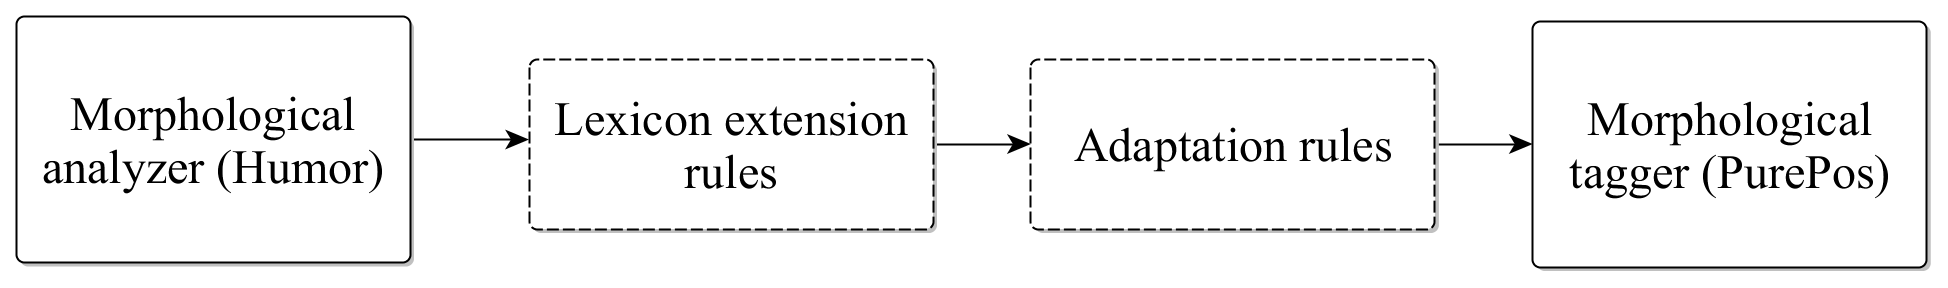
\includegraphics[scale=0.2]{MorphComplexity/mlu_architecture.png} 
  \caption{The architecture of the morphological tagging chain adapted for the HUKILC corpus}
  \label{fig:speech-tagger}
\end{figure}


In order to apply a \acrlong{ma} prepared for written texts, its analyses had to be adjusted for the transcripts. 
Thus, adaptation rules -- based on regular expressions and domain-specific word lists -- were constructed using the development set.
Their formulation could be done with high confidence, since most of the transcripts contained controlled conversation covering only a few topics. 

As a first step, morphological analyses of about 40 words typical of spoken language were created manually. 
These tokens were mostly interjections not used in written language (such as \textit{hűha} `wow’), while some adverbs were regarded as utterance words in the corpus (e.g. \textit{komolyan} `seriously’). 
Furthermore, those tokens that are written as one word in transcripts but are spelled as two words in formal texts were also added to the lexicon. 
An example is \textit{légyszíves} `please’ which is written formally as \textit{légy szíves}. Finally, diminutive analyses were also provided where it was necessary. 
E.g. \textit{kutyus} `doggy’ was also analysed as \textsc{n.dim} with the lemma \textit{kutya} `dog’ beside the old label \textsc{n} and the \textit{kutyus} `doggy’ root. This process was carried out by investigating the lemmata produced by Humor: if the deletion of the derivational affix resulted in a root enumerated in a domain-specific list, a new diminutive analysis was created as well. 

Concerning the disambiguation process, PurePos was extended with rules to adapt its knowledge to the target domain. 
First, the tagger was forced to assign diminutive analyses when it was possible. 
Secondly, rules were developed to assign interjection and utterance annotations for appropriate words.
Finally, further enhancements were carried out by investigating the common mistakes of the tool on the development dataset.

A frequent error of the chain was the mistagging of \textit{akkor} `when’ and \textit{azért} `in order to’. 
These words are pronouns and can be categorized as either adverbial, noun phrase level or demonstrative ones, and can also behave as pronomial adjectives. 
Generally, when \textit{akkor} is followed by \textit{amikor} `when’ (as in \textit{Akkor érkezett meg, amikor mentem} `He arrived, when I left’) and when \textit{azért} is followed by \textit{mert} `because’ (as in the sentence \textit{Azért eszik, mert éhes} `He eats, because he is hungry’) these pronouns are demonstrative ones. 
Furthermore, such co-occurances are more common in the transcripts than in the Szeged Corpus, since they are frequently used during reasoning or telling a story. 
As these long-term dependencies could not be learnt by the trigram tagger applied, rules were employed to tag these tokens correctly.

The next issue was the case of the word \textit{utána} `afterwards, then; after him/her/it’. 
It can either be used as an adverb of time (as in the sentence \textit{Utána elindultunk} `Then we left’) and as a postpositional phrase meaning `after him/her/it, following him/her/it’ (as in \textit{Elindultunk utána} `We went after him’). 
The former usage is more frequent in spoken language: when this word is directly followed by conjunctions such as \textit{meg} `and’ or \textit{pedig} `however’, it is always an adverb. 
Therefore, \textit{utána} was tagged as an adverb in the transcripts when it is followed by one of these trigger words. 

The last rule introduced deals with \textit{meg}, which may function as a verbal prefix or as a conjunction.  
Moreover, it is usually an expletive in spoken language.
Therefore, the conjunctive label was assigned to the word when there was not any verb in its two token window.

\section{Computing morpho-syntactic complexity}

As a first step, general principles of counting morphemes were established. 
In a language with such a rich derivational system as Hungarian, it is often very complicated to identify the lemmata. 
This is even more difficult in our case, since no common methodology exists to determine the boundary of productivity in child language. 
This was based on studies of Brown \cite{Brown1973}, Retherford \cite{retherford1993guide}, Wéber \cite{Weber2011} and Réger \cite{Reger1990}, with some necessary modifications. 
The basic principles were: 
\begin{enumerate}
 \item only meaningful words were analyzed, thus fillers (filled pauses such as \textit{ööö} `er’), punctuation marks and repetitions are not counted in the utterances;
 \item phatic expressions (e.g. \textit{igen, mhm} `yes, uhm’) serving to maintain communication and not conveying meaning were omitted;
 \item inflectional suffixes and lemmata were each counted as one unit; 
 \item derivational morphemes (including diminutives) were not counted as separate ones,
 \item reciprocal and indefinite pronouns (e.g. \textit{minden\#ki} `everybody’) and compound words (such as \textit{kosár\#labda} `basketball’) were counted as one morpheme.
 \end{enumerate}
 
Following the guidelines of Brown \cite{Brown1973}, proper names (such as \textit{Nagy Béla}, \textit{Sári néni} `Miss Sári’) and lexicalized expressions (e.g. \textit{Jó napot} `Good morning’), which are frequent in speech, were also considered as one unit. 
Their identification was carried out employing rules. 
For this, the method relies on capitalized token sequences and a domain-specific list of words.

As for the automatization of rules, they were implemented using the morphological annotation of the corpus. 
First, each item on the list of fillers was eliminated.
Afterwards, tagged words known to the \acrshort{ma} were split into morphemes by the Humor analyzer. 
If more than one analysis was created for a word, the least complex one was chosen, since analyses only differed in the number of derivative tags and compound markers (which we previously decided not to count) in the majority of the cases.
As the labels of the annotation scheme were composed of morphemic properties, the estimation of unknown words could be based on their tags. 
Therefore, such calculations were carried out counting only the inflection markers in the guessed tags (as it is listed in principles above). 

\section{Evaluation}

First of all, morpho-syntactic tagging performance of the system was investigated. 
%For this, we calculated precision per token not counting punctuation markers (cf. Section \ref{}).
Full analyses -- containing both the lemmata and the tag -- were compared to the gold standard data, not counting punctuation marks and hesitation fillers.

\begin{table}[H]
\centering
\caption{Evaluation of the improvements on the tagging chain (test set)}
\label{tab:eval_tag}
\begin{tabular}{ l r r} 
\hline
\multicolumn{1}{l}{\multirow{2}{*}{Morph. tagger}} & \multicolumn{2}{c}{\hspace{0.8cm} Tagging accuracy} \\
& Token &  Sentence \\
\hline
Baseline &  \hspace{0.8cm} 91.97\%  & \hspace{0.8cm} 68.37\% \\
\hspace{0.2cm} + DIM &  94.92\% & 79.96\% \\
\hspace{0.2cm} + CONJ & 95.53\% & 81.74\% \\
The full chain & \underline{96.15\%} & \underline{83.96\%} \\

\hline
\end{tabular}
\end{table}

For measuring the individual advances of the enhancements presented, four different settings were evaluated on the test set. 
The first was a baseline using raw analyses of Humor disambiguated by PurePos. 
The second system (DIM) employed the extended vocabulary and handled the diminutive analyses as described in Section \ref{sec:tagging}. 
The next one -- marked with CONJ -- utilized further rules aiming to tag \textit{azért} and \textit{amikor} correctly. 
Finally, the last system presented contains all the enhancements detailed above.

Measurements in Table \ref{tab:eval_tag} show that the baseline tool tagged erroneously 3 out of 10 sentences. 
On the contrary, each of the enhancements improved the overall performance significantly.
For this, we used the Wilcoxon matched-pairs signed-rank test at p<0.05. 
Furthermore, results indicate that the accuracy of the adapted chain is comparable with that of the tagging methods for written corpora \cite{zsibrata2013magyarlanc}. 

As for the \acrshort{mlu} estimation task, two metrics were used for the evaluation. 
First, \acrlong{mre} was calculated (as in \cite{Witten2011}), comparing the $a_i$ manual morpheme counts with $p_i$ predicted values for the $i$th utterances:
\begin{equation}
MRE = \sum_{i=1}^n \frac{|a_i-p_i|/a_i}{n}
\end{equation}
This measurement shows the average relative deviation of the estimated morpheme counts from the one of human annotators. 

In addition, Pearson's correlation coefficient\footnote{The notation is the same above, except $\overline{x}$ is the average of $x_i$ values and $n$ denotes the total number of observation.}
 \eqref{eq:corr} (cf. \cite{Witten2011}) was employed as well:
  \begin{gather}\label{eq:corr}
  \frac{S_{PA}}{\sqrt{S_P S_A}} \text{, where } \\
  S_{PA} = \frac{\sum_i{(p_i-\overline{p})(a_i-\overline{a})}}{n-1} \text{, } \nonumber \\
  S_{P} = \frac{\sum_i{(p_i-\overline{p})^2}}{n-1} \text{ and } S_{A} = \frac{\sum_i{(a_i-\overline{a})^2}}{n-1}  \nonumber
  \end{gather}
  indicating the correspondence between the output of the processing chain and the counts of human annotators.


\begin{table}[H]
\centering
\caption{Evaluation of the  \acrshort{mlum} estimation algorithm using the output of  different morphological taggers}
\label{tab:eval_est}
\begin{tabular}{ l r r} 
\hline
Morphological tagger & \acrshort{mre} & Correlation \\
\hline
The baseline tagger &  0.1325  &  0.9612 \\
The adapted tagger & \underline{0.0449} & \underline{0.9901} \\
Gold standard annotations &  0.0279 &  0.9933 \\
\hline
\end{tabular}
\end{table}

Since both metrics require a gold dataset, morpheme counts were manually calculated for 300 utterances of the test set.
Table \ref{tab:eval_est} presents the evaluation of the \acrshort{mlum} estimation algorithm on this manually checked corpus. 
First, we evaluated the output of the baseline tagger with our morpheme counter. 
Beside this, both the gold standard data and the output of the enhanced tagging tool were used as an input of the estimator. %enabling a detailed comparison of enhancements presented. 
On the one hand, these results can be interpreted as an in vivo evaluation of the adapted tagger showing significant improvements over the baseline.
On the other hand, it was found that the overall performance of the estimation methodology is outstandingly high.  
The high correlation of the automatic chain indicates that our method can properly measure the morpho-syntactic complexity of Hungarian spoken language in practice. 
Therefore, the time-consuming manual counting procedure can be replaced with the proposed method.